\documentclass[twocolumn,english]{IEEEtran}
\usepackage[T1]{fontenc}
\usepackage[utf8]{inputenc}
\usepackage{babel}
\usepackage{amsthm}
\usepackage{graphicx}
\usepackage{epstopdf}
\usepackage{color}
\usepackage[unicode=true,
 bookmarks=true,bookmarksnumbered=true,bookmarksopen=true,bookmarksopenlevel=1,
 breaklinks=false,pdfborder={0 0 0},backref=false,colorlinks=false]
 {hyperref}
\hypersetup{pdftitle={Unified Transport Stack for Cloud Computing},
 pdfauthor={Mathias Hablützel},
 pdfpagelayout=OneColumn, pdfnewwindow=true, pdfstartview=XYZ, plainpages=false}

\makeatletter

%%%%%%%%%%%%%%%%%%%%%%%%%%%%%% LyX specific LaTeX commands.
\DeclareRobustCommand*{\lyxarrow}{%
\@ifstar
{\leavevmode\,$\triangleleft$\,\allowbreak}
{\leavevmode\,$\triangleright$\,\allowbreak}}
%% Because html converters don't know tabularnewline
\providecommand{\tabularnewline}{\\}
%% A simple dot to overcome graphicx limitations
\newcommand{\lyxdot}{.}


%%%%%%%%%%%%%%%%%%%%%%%%%%%%%% Textclass specific LaTeX commands.
 % protect \markboth against an old bug reintroduced in babel >= 3.8g
 \let\oldforeign@language\foreign@language
 \DeclareRobustCommand{\foreign@language}[1]{%
   \lowercase{\oldforeign@language{#1}}}
\theoremstyle{plain}
\newtheorem{thm}{\protect\theoremname}
\theoremstyle{plain}
\newtheorem{lem}[thm]{\protect\lemmaname}

%%%%%%%%%%%%%%%%%%%%%%%%%%%%%% User specified LaTeX commands.
% for subfigures/subtables
\ifCLASSOPTIONcompsoc
\usepackage[caption=false,font=normalsize,labelfont=sf,textfont=sf]{subfig}
\else
\usepackage[caption=false,font=footnotesize]{subfig}
\fi
\makeatother

\providecommand{\lemmaname}{Lemma}
\providecommand{\theoremname}{Theorem}

\addtolength{\textheight}{-2cm}
\addtolength{\topmargin}{1cm}
\addtolength{\columnsep}{1cm}

\begin{document}

\title{Unified Transport Stack for Cloud Computing}

\author{Mathias Hablützel \thanks{Hablützel is with Zürcher Hochschule für Angewandte Wissenschaften, Institut für
    angewandte Informationstechnologie, Winterthur, Schweiz, EMail:
    \protect\href{mailto:mathias.habluetzel@zhaw.ch}{habl@zhaw.ch}.
    }
}


% \IEEEspecialpapernotice{Invited Paper}


%\IEEEaftertitletext{after title text like dedication}


%\markboth{Journal of XXX}{Your Name \MakeLowercase{\emph{et al.}}: Your Title}


\IEEEpubid{0000--0000/00\$00.00~\copyright~2007 IEEE}
\maketitle
\begin{abstract}

\end{abstract}
\begin{IEEEkeywords}
network, transport, unified transport, communication
\end{IEEEkeywords}

%%%%%%%%% LAYOUT %%%%%%%%%%
% 1. Motivation / Problem Statement
% 2. State of the Art / related Work
% 3. Contribution / What's new
% 4. Evaluation and Results
% 5. Conclusion and Outlook
%%%%%%%%%%%%%%%%%%%%%%%%%%%

\section{Introduction}

\IEEEPARstart{W}{orking} with network transport protocols and built-in
libraries either provided by the operating system itself or by third party
libraries, a developer is usually confronted with a series of cryptic options,
settings, flags and syscalls. This renders the task of writing understandable
code not only difficult but also a matter of experience, but also slows down
the job of researcher when they want to develop new protocols. Plus, the
effort needed to just send a first datagram is significant and leads to
bloated source code with several hundred lines of code just for the
initialization matters.

Furthermore most used implementations are heavily operating system dependent
therefore creating an overhead in de facto re-writing or re-implementing large
portions of the network code for other protocols and/or other major platforms.
If you simply consider the POSIX network style as used in *nix systems like
Linux, *BSD, OSX and similar derivatives you are confronted with different
level of POSIX ranging from 4.xBSD to POSIX.1-2008 with operating system
flavored variants or even compiler and standard library flavored extension
which literally render the code an obscure conglomerate.

When a developer writes a distributed application he will choose a stack and
write his code against this API. Altering the chosen stack on a later date
implies to also rewrite portions of the code which handles the multiplexing,
memory and communication paradigms. Also if the developer chooses to use
several stacks which meet the requirements this inevitably brings in a lot of
redundant code and a potential field of mistakes due to duplication.

As a last point to be stressed, adding a new family of protocols by using a
third party library usually introduces a new paradigm of how things are
handled. This may range from threading to passing-by-reference or by-value or
even different ways of how the memory content is shoved around, either by a
pair of pointer and length value or by an object like a vector, or even
non-uniform function/method naming. This all increases the time a developer
needs to learn a new library and therefore is an opportunity not only to
increase productivity but also by allowing to easily add new protocols by
writing a wrapper according to the south bound API provided and required by
this later proposed unified network stack.

In a later point it is possible to even extend the stack with intelligent
algorithms which choose the appropriate (or read "best, most adapted")
protocol complying to the developers before-stated requirements according to
the network or path health, status, situation and circumstances.

So the aim of developing a unified network stack is not to design a solution
which does everything possible innately (it speaks the most prevalent
protocols), but is able to do so by providing an uniform skeleton for
extensions. In a later step this framework may be directly integrated into
core network functionalities of operating systems or as an extension, and the
developer may then just provide his extension (read a new protocol) to the
core and therefore be confident that when sticking to certain dogmas the
protocol should run on widely spread systems, even if the system is not open
sourced.

\section{Previous Work}

\subsection{Boost.Asio\cite{boost.asio}}
Boost is a widely used general purpose library that among others provides
networking functionalities as Boost.Asio with a focus to be very strong
cross-platform and usually is provided in many unixoid systems with their
respective package manager.

It provides building blocks for I/O (input, output), concurrency and signaling
but is not designed to provide a framework which may be easily extended by the
application developer. The built-in crypto support relies on OpenSSL which one
may consider problematic since SSL is built upon hierarchical certification
authorities.

Asio provides timers which are handy for real-world networking application but
also may be an indicator or an unwanted motivation to choose bad paradigms.
The most common layer 4 protocols TCP, UDP and ICMP are supported but the
developer is also entitled to access a raw socket.

The use of streams make the use of these sockets very easy and straightforward
with all following advantages std::ios brings. The authors of Boost.Asio state
that the strong type safety C++ enforces is an advantage to the loosely
integer typed BSD socket handles. This is partially true, you are able to
build a object with further information about the socket but eventually the
integer typed handle is nothing more than a operating system provided
reference and therefore also an issue to be addressed by the operating
systems.

\subsection{ZeroMQ\cite{zeromq}}
This is a message queueing library which out-most strongly focuses on message
and communication patterns and paradigms. It uses a well documented internal
format ZMTP with no prevalence in other stacks and therefore is little
interoperable with established services like webserver (HTTP) provide.

ZeroMQ is a toolkit which provides building blocks for creating new
decentralized and distributed communication patterns with no interest in
providing an extendable framework like construct for new protocols even though
it supports the most used of transport protocols like TCP, UDP, IPC, inproc
and PGM. It is a message handling library and not designed to add a developer
invented chain of protocols. Extensions provide crypto extension via the NaCl
protocol engineered by D.J. Bernstein, Tanja Lange and Peter Schwabe.

\subsection{cpp-netlib\cite{cpp-netlib}}
This library coming from Google engineers depends fully on Boost and actually
is an extension to add HTTP. It doesn't add any other transport or application
protocols and is therefore an interesting library if the application already
uses Boost.

The message template\cite{cpp-netlib-message} appears to be complete for
protocols similar to HTTP even though it's a very lightweight construct. For a
very flexible approach to add custom functions that manipulate messages
so-called directives are used, unfortunately a very complicated and confusing
approach but providing a powerful chaining mechanism known from
streams\cite{cpp-netlib-directives}.

Summarized this library provides functions for HTTP and URI parser in C++
which integrates well with prevailing Boost usage even though it requires a
high set of C++ skills to implement and extend the framework.

\subsection{POCO C++ Libraries\cite{poco}}
The tagline introduces POCO as a library and framework for network and
internet-based applications. The simplistic approach of providing as much as
possible but not everything if the last 5 \% of completeness would make 95\%
of the code volume is bracing. POCO is explicitly aimed for middleware usage.

The wide range for application protocols\cite{poco-network} and also providing
precast blocks for HTTP server and client, POP3 and SMTP clients as well
support for sockets and raw sockets shows very well what purpose this library
wants to fulfill.  Furthermore the it provides stream classes for Base64 en-
and decoding, DEFLATE de- and compression and crypto is done with NetSSL. The
approach of using STL streams renders the chaining of several stacks and
parser very easy, plus the integrated HTML form support directly allows to
talk to web services originally aimed for human interaction.

An integrated framework for multithread processing of TCP connections via
instantiating a TCPServerConnection for every accepted connection may lead to
considerable thrashing and a concept for reusing objects should be considered.

The POCO C++ library focuses on widespread protocols while providing functions
for retrieving information and data from the several layers of communication
protocols. The small footprint makes it interesting for use in embedded
systems and therefore also for the Internet Of Things which need to talk to
REST services.

\subsection{ACE - The ADAPTIVE Communication Environment\cite{ace}}
Started as an academic project ACE has the strongest focus on patterns of all
these libraries and provides a limited range of supported protocols (TCP, UDP
and ATM) without considering any upper application layer protocols like HTTP
nor providing handy STL stream oriented classes. Furthermore it is not thought
to have a framework for extensions and therefore is harder to extend with
developer submitted functionalities.

The aim of this stack is primarily for industrial application (like
satellites) which need a extraordinary robust and reliable communication stack
without providing any marshalling. Also the good coverage and abstraction of
mutex, semaphores and threads is intended for parallelized applications with
shared memory.

\subsection{yield\cite{yield}} 
Unfortunately this library only has one committer, no documentation and many
bugs have been left unresolved for years, so this seems to be more an
enthusiasts work and shared to who would be interested in. It's merely a C++
wrapper around POSIX sockets and doesn't provide much more than the usual UDP
and TCP and leaves the impression to be more of a wrapper than a toolkit.

\subsection{RakNet\cite{raknet}}
Unfortunately this library is not opensourced though it has some
Indie-Licenses for enthusiast wanting to write a game and therefore provides a
lot more than just the needed network stack, toolkit and framework. It is best
described as a game middleware.

\subsection{WvStreams\cite{wvstreams}}
Another seemingly dead project, the description was unavailable in January
2014 and was retrieved through archive.org. Apparently the last commit
occurred over three years ago in April 2011. According to the description
dating from 2004 this is basically a C++ wrapper doing the usual syscalls for
I/O reducing the amount of lines to write when doing the standard networking
operations and other repetitive tasks. Sadly this library provides relatively
few network related functions.

\section{Proposition}

The proposed architecture (figure \ref{fig:arch-overview}) consists of three
main components: Helper functionalities for threading, timers, SDN controller
and other patterns; the individual building blocks providing support for
different network protocols, crypto and parsers; and finally the network block
which acts as an intelligent service provider handling all the internal
configuration and de facto is an opaque structure to abstract.

\begin{figure}[h]
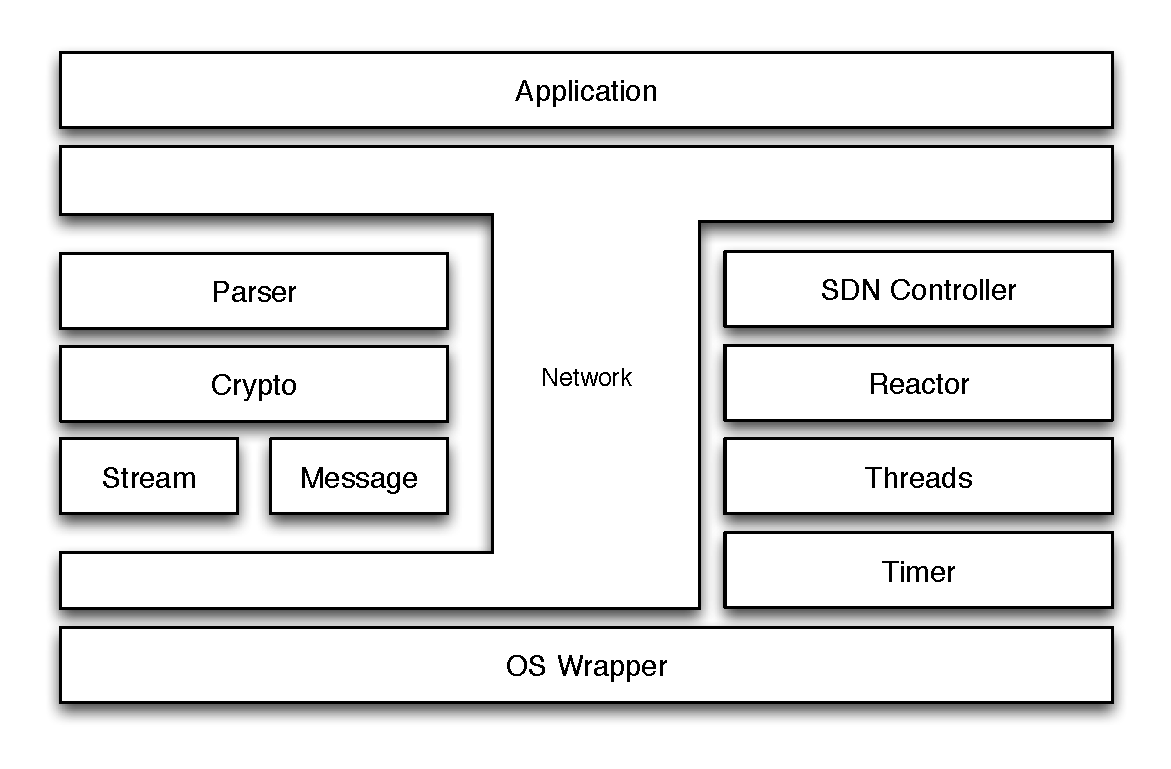
\includegraphics[width=\columnwidth]{Architecture_overview.eps}
\caption{Architecture overview -- this diagram shows that the parser, crypto,
stream and message blocks are separate building blocks which are
interchangeable or omitable.}
\label{fig:arch-overview}
\end{figure}

The architecture provides not only a northbound API to the developer but also
a southbound internal API for adding new blocks for extending the supported
protocols. Common protocols like UDP, TCP or ICMP must be built-in since the
vast majority of application generated traffic is handled by these (around 79\%
TCP and 19\% UDP traffic was measured on September 17--18 2011 at an IX in
Chicago run by Equinix\cite{caida:application-protocol-percentage}). Also it
would be very helpful to provide several other protocols for a steganographic
transport of data\cite{ijcsi:dns-steganography} to evade deep packet
inspection and censorship.

An easy setup, configuration and simple usage is of outmost importance to
prevent many opportunity for mistakes and errors. Also a very clear
hierarchical composition of the different parts helps to understand how things
work.

\begin{figure}[h]
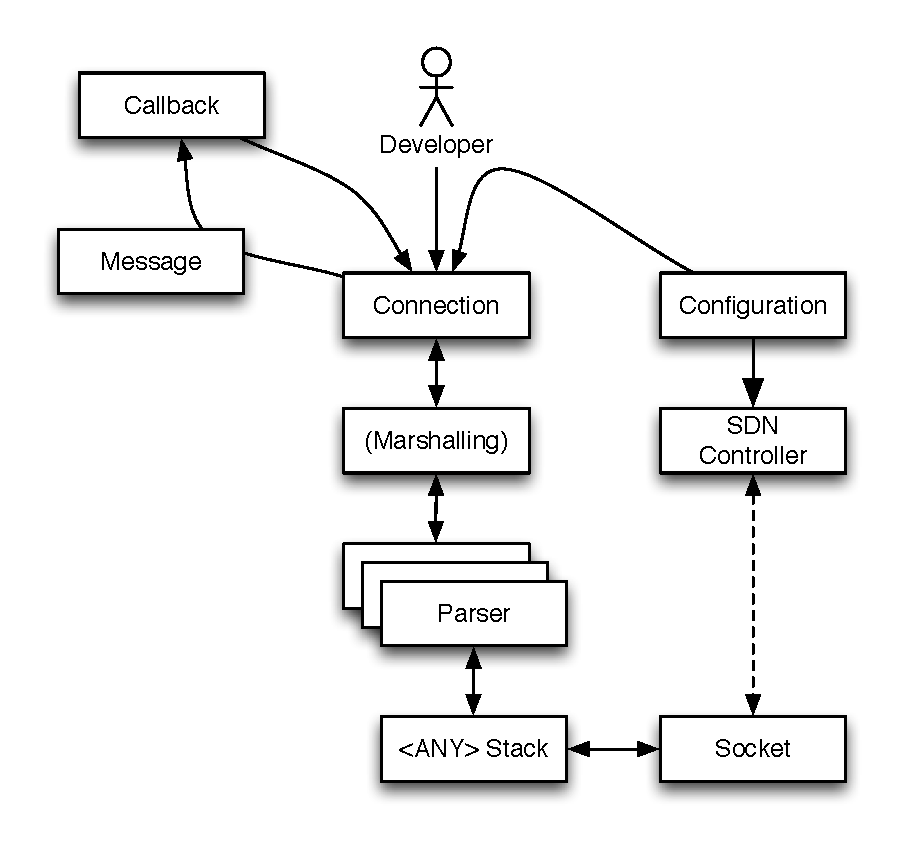
\includegraphics[width=\columnwidth]{Concept.eps}
\caption{Very coarse overview about how the different elements interact with
each other. The developer essentially creates a connection object and
indicates the wanted configuration and a callback. Then the connection will
setup everything as required and pass incoming messages to the callback. The
marshalling, parsing etc. is done transparently.}
\label{fig:concept}
\end{figure}

\subsection{Specific requirements}

First of all since this transport stack is aimed to be integrated into
different operating systems the choice of a programming language is naturally
narrowed down to the classic machine-oriented languages and here I choosed C99
and C++11. This allows to use C++ stream operators and this constitutes of an
simple way for chaining stacks or parser for I/O, along with providing access
to the several layer of communication.

Since the rise of multi-core architectures in
2004\cite{amd:first-multicore-x86} the need for concurrency pattern is without
doubt widely necessary. In this terms providing support for concurrency
patterns like mutex, locking and semaphores surely is a big help to an
engineer. Plus adding templates for patterns like reactors, proxy or singleton
will provide a big help for repetitively used code.

In times where networks are not necessarily physically wired paths SDN
(Software Defined Networking) is an important topic for service providers as
Cloud Computing PaaS is. The idea behind this SDN controller is to be able to
set certain requirements about the route and the developer has not to care
about network configuration and setup.

Newer protocols like SCTP and DCCP are usually first supported by opensource
operating systems which have a leading market share in the server
domain\cite{w3techs:os-web}, and lacking in closed source though market
relevant, turn the task more difficult to spread new technologies especially
when the user end support is lacking\cite{netmarketshare:desktop-os}. Here
also this proposed stack is revolutionary since it would enable the developer
to write new protocols for several operating system at once and by this way
spread new technologies faster without intervention needed by the vendor.

\subsection{Proposed extensions to existing stacks}

In a world of near-pervasive computing with wearables collecting sensitive
personal and even medical data transporting the data in a safe manner becomes
crucial. Not only to prevent tampering of potentially critical data (imagine a
cardiac pacemaker) but also to protect the transmitted content (imagine
mobile-banking orders). Therefore I strongly suggest to implement many
cryptographic stacks like IPsec, NaCl, SSL and RSA but to avoid cryptographic
primitives like 3DES, AES, MD5 or SHA1 to prevent developers from building
their own cryptography.

One big challenge for mobile devices is dealing with the scarce resource of
electricity and bringing support to handle this is a welcome opportunity to
demonstrate the possibilities of this stack. It may be imagined an application
polling informations in the background may want to schedule this job when the
system is anyway awake and avoid to wake up the components from their deep
sleep, and by this reduce the battery drain when not used. Figuring out when
the system is in which state and handling this different cases right (you may
want an instant messenger to use push services and retrieve the data also when
the system is mostly off, whereas a feed reader may want to fetch the data
only when the device is awake or on demand) is a challenging task. A system
providing many different use cases explores new possibilities for extending
autonomy.

Companies with BYOD (Bring Your Own Device) policy and smartphone
manufacturers will face the challenge to change this situation into JOC (Join
Our Cloud) when statistically 1.3 devices are owned per
household\cite{gartner:predicts-2014-cognizant-computing}. The idea of JOC is
to define a domain with given restrictions and requirements which the device
has to adhere. Now if the developer can just state that the traffic to the
endpoint has to satisfy certain parameters (for instance every connection
requires an up and running VPN connection before any data is sent by the
application) and the stack takes care of the rest the risk of wrong security
is reduced.

For societies living in a deeply dependent way of communication resilience to
interruption is crucial. Consequently the stack should support ad-hoc mesh
network self-configuration and a wide variety of peer-to-peer protocols like
bittorrent. This may provide an uninterruptible service for first responder
teams in emergency cases where the prevailing infrastructure collapsed or was
severely damaged.

The published market forecast by Frost \& Sullivan in July
2009\cite{frost:iptv-market} stated that by end of 2012 approximately 140 mio
customers will consume broadcasts via IPTV. But ABI research states that
broadcast providers reached over 900 mio customers in
2013\cite{abi:iptv-marketshare} and this clearly shows the impact multicast
stream traffic has on the network.  Therefore adding functionality for
broadcasting such content is surely an interesting opportunity but support for
receiving such broadcasts may turn every device in an IPTV broadcast
consummation device. The next consistent step would be to integrate an
intelligent core which detects roaming and quickly buffers to avoid a stream
interruption when handing over to another cell. Also providing intelligent
multi-homing support for changing from cell-radio connectivity to a more
stationary wifi connectivity without interruption is a feature with market
value.

In a last point I want to suggest to add functionality for forcing devices to
switch the cell-tower allowing the providers to balance the load more equally
or to provide better connectivity to a weaker uplink even though the
communication module would usually choose the strongest signal over good link
quality.

\section{Discussion}

Having a dedicated transport stack is of course very handy and improves a lot
of factors when the developer does not have to include a whole library like
Boost and by this can reduce not only the dependencies, unused libraries (or
at least pieces of it) and compile time. Furthermore a very flexible and
modular approach is not only en vogue but also necessary to provide a
made-to-measure service for the developer and also allows to extend the stack
as wished.

C++ streams known from the Standard Template Library are a very easy way to
chain several parsers working on \texttt{std::vector} or \texttt{std::string}
but they also bring in some potential for conflicts, hard to understand code
and misuse. As stated by the internal styleguide provided by
Google\cite{google:cpp-styleguide} streams favor especially dereference
mistakes and also it is subject to controversy if overloading is a good
habit.

Overloading for the sake of using this languages feature is certainly wrong
and it should be used very defensively. I don't consider it to be harmful if
used wisely and in the right situation, so overloading \texttt{operator<<}
should be restrained to parsing functionalities which each extract the
payload and return a new object of the same type as the input with the copied
payload.

In times where higher demands of confidentiality, privacy and
non-repudiation or exactly the opposite confidentiality, privacy and
\emph{repudiation} providing support for cryptographic protocols is heavily
encourage and somewhat a necessity. But there lie two major pitfalls, first
of all a developer is not a cryptographer and therefore should not under any
circumstances do cryptography (or even be enabled to do so by the
framework)\cite{pzimmermann:introtocrypto}.

My second major concern is that a vulnerability or a bug may lead to a
widespread required update if for instance this library is deployed in
embedded devices thousandfold. In a last point I'd like to also mention that
interoperable cryptography is essential and requires special attention and
testing, especially edge cases.

For a developer it is easier to extend and reuse something existing. Since it
allows to use other building blocks and therefore already provide a fully
featured environment even though the novelty may consist of a few lines of
code.

Providing an open extendable stack may also entitle developer to commit and
provide new code which in a later moment will go upstream. This situation is
like a giant reactor and incubator for new ideas and opportunities as other
projects like Linux showed.

But this is also a potential source of problems when this stack starts to
reimplement pieces of code already existent in the kernel or other
core-libraries. Plus including everything possible in a stack is a mixed
blessing, the stack is able to do everything but tends to be bloated with things
developer will rarely use. The challenge here is to find the right balance.

In a further point this stack is a new way of adding developer added value in
terms of transport protocols to for example a cloud instance running an
application. So basically a cloud application computing power provider
enables the developer to add his extensions to the transport stack and
therefore adapt the communication directly to his needs.

On the downside this may implicate an immense risk since some extensions may
not only require full access to the kernel-land and total control down to the
NIC, but also may be used to directly attack the infrastructure in non
foreseeable ways, especially with attempts to break out from the jailing.

This stack enables applications and software to become QoS aware and
explicitly ask for a certain setting of configurations on the network.
Therefore an application for VoIP can state that the link may not require a
lot of bandwidth but a low latency and few packet loss.

Mesh networks as known from several rural provisioning in South Africa by
residents and also from the OLPC (One Laptop Per
Child\cite{olpc:meshnetwork}) project are not of real interest in first world
countries since the pre-existing infrastructure covers the daily need better
than a fluid setup which needs to reconfigure itself often. But on the other
hand this static infrastructure is vulnerable to interruption, failure and
deliberate harm since it is usually very centralized.

Also many emergency relief organisations have to first bring in communication
equipment (handset, relais, antennas etc. pp.) for their need which delays the
organisation of help substantialy. Therefore providing a self organising mesh
based network which could make use of mobile handsets already on site can
prove itself as very advantageous when transportation means are a severe
problem.

GSM (3GPP) already supports handover from cell tower to another tower, A.
Sarma, S. Joshi and S. Nandi explain very well an extension for IEEE 802.11 in
their paper \cite{ijcn:ieee80211-handover} (described in figure
\ref{fig:handover}) even though this is aimed at IEEE 802.11 and not at 3GPP.
Originally, handover induced by the the base station is not intended by the
standard therefore the stack would have to actually extend the PHY layer and
possibly break compatibility with the existing hardware and devices. In IEEE
802.21 it is even described for vertical handovers (for example from IEEE
802.11 to 802.16 respectively Wifi to WiMAX) but has so far not reached any
relevance.

\begin{figure}[h]
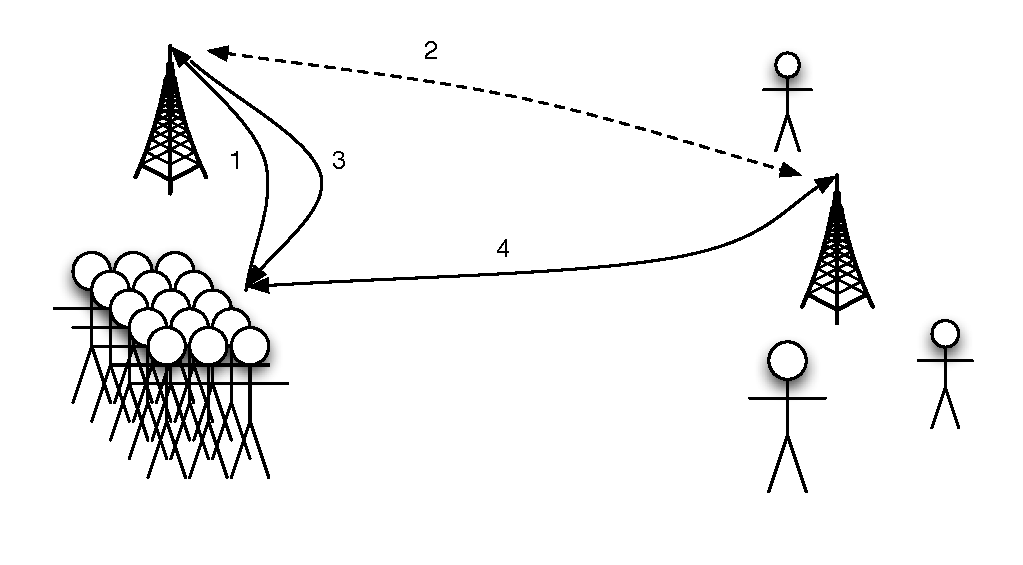
\includegraphics[width=\columnwidth]{Handover-to-less-frequented-cell.eps}
\caption{When the CPE experiences serious degradation in QoS it shall send a
list of visible BTS [1] to the currently connected BTS. This BTS will then
lookup what other BTS could handle the client[2] (I would like to extend this
to according to it's load parameter and connection requirements), then
signaling to the CPE which BTS to connect to[3] and eventually the CPE
connects to the less busy BTS[4] if possible (read: without dropping
connections).}
\label{fig:handover}
\end{figure}

A further very welcome improvement for engineers and developer is to be able
to reuse paradigms, patterns and templates and reducing by this the overhead
of rewriting them. But writing too general constructs for supporting the
widest range possible of developer engineered code can turn these helper
functions into a hard to understand and complex templating and can be
considered harmful. Therefore a careful balance or different specific types
implementing these patterns, paradigms and templates may be required and well
adapted for the purpose.

The central configuration passed to the communication class is to be thought
as a middleware like construct since the intelligence is in this
class. This means that a lot of crucial code is in one place therefore
reducing the spread but also bloating one class in this case. I suggest to
use a inheritance or derivation based approach for a cleaner outline.

Protocols like HTTP require session handling, especially on the server side
which needs special attention. Challenges like lease times of sessions are
not subject to developer but rather are a topic system operators have to
tweak and therefore should not have to be taken care of by developers. This
problem statement is subject of subsequent work.

Also many security issues of such a stack are not considered and not matter
of this subject here. I believe that this topic requires a more in depth
knowledge than required for a generalistic enabler for several transport
means as I want to provide in this and future work.

In a last point, this stack has not been designed for massive parallelism and
concurrent computing like a machine mit GPGPUs would be able to do so. But by
providing mechanism like mutexes, semaphores, locks and queues a lot can be
done for multicore architectures that are current as in early 2014. But for
the long term future with hundreds of processing units this stack may turn out
to be not ideal.

\section{Conclusion}

I showed an outline of a new plugable stack which enables a developer to
rapidly add their value and protocols for a future generation of cloud based
and SDN-enabled applications. In a later section I critically discussed and established
a base for my design decision.

\section{Results}

\textbf{Results will be a newly designed stack for communication in C++11 and
C99 and matter for subsequent research and implementation.}

\section*{Acknowledgment}

A lot of this work is due to three (anonymous) personal friends of mine, Dmitri
Rubinstein (with the DFKI) for his hour long support and discussions, Philipp
Aeschlimann whos great ideas about SDN formed an important foundation and
Andy Edmonds (both with the ZHAW) whos expertise in writing helped to get
this idea on paper.

\bibliographystyle{IEEEtran}

\bibliography{IEEEabrv,IEEEexample,literature}

\begin{IEEEbiography}[{\includegraphics[clip,width=1in,height=1.25in,keepaspectratio]{Portrait_placeholder.png}}]
{Mathias Hablützel} was born in Switzerland in 1989 and pursued a bachelor
degree in applied computer science at the Zürcher Hochschule für Angewandte
Wissenschaften with focus on network communication. After his graduation he
started his career as a researcher at the ICCLab at the ZHAW. His particular
personal interests are Linux, net- \& compsec, cryptography and steganography.

\end{IEEEbiography}

\end{document}
